\documentclass[
  11pt,
  letterpaper,
   addpoints,
   answers
  ]{exam}

\usepackage[utf8]{inputenc}
\usepackage{../exercise-preamble}
\usepackage{float}
\usepackage{subcaption}
\usepackage{pgfplots}
\pgfplotsset{compat=1.18}
\usepgfplotslibrary{groupplots}
% TikZ libraries needed for `right=.. of ..` and coordinate math
\usetikzlibrary{positioning,calc,arrows,arrows.meta}

% Configuración de numeración de páginas
\makeatletter
\def\@oddfoot{\hfil Página \thepage \hfil}
\def\@evenfoot{\hfil Página \thepage \hfil}
\def\@oddhead{}
\def\@evenhead{}
\makeatother

\begin{document}

\noindent
\begin{minipage}{0.47\textwidth}

\includegraphics[width=\textwidth]{../fcfm_die}
\end{minipage}
\begin{minipage}{0.53\textwidth}
\begin{center} 
\large\textbf{Análisis de señales} (EL3203-2) \\
\large\textbf{Clase auxiliar 4} \\
\normalsize Prof.~Jorge Silva.\\
\normalsize Prof.~Aux.~Erik Sáez
\end{center}
\end{minipage}

\vspace{0.5cm}
\noindent
\vspace{.85cm}
%----------------------------
\noindent\rule{\textwidth}{0.4pt}
\subsection*{Análisis de Fourier: para Señales Continuas y Discretas}

El análisis de Fourier constituye el fundamento teórico para la descomposición espectral de señales, abarcando tanto el dominio continuo como el discreto. Las cuatro herramientas principales \textit{(Serie de Fourier, Transformada de Fourier, Serie de Fourier Discreta y Transformada de Fourier Discreta)} abordan diferentes combinaciones de periodicidad y naturaleza temporal, proporcionando una base completa para el análisis frecuencial.

\subsubsection*{Serie de Fourier: Señales Continuas Periódicas}
La serie de Fourier descompone señales continuas y periódicas de período \(T\) en una suma discreta de armónicos:
\begin{equation}
x(t) = \sum_{k=-\infty}^{\infty} c_k\,e^{jk\omega_0 t}, \qquad \omega_0 = \frac{2\pi}{T}
\end{equation}
Los coeficientes complejos se calculan mediante:
\begin{equation}
c_k = \frac{1}{T}\int_{t_0}^{t_0+T} x(t)\,e^{-jk\omega_0 t}\,dt
\end{equation}

Características principales:
\begin{itemize}
\item \textit{Dominio temporal}: Señales continuas y periódicas (potencia finita, energía infinita)
\item \textit{Dominio frecuencial}: Espectro discreto con componentes en \(k\omega_0\)
\item \textit{Coeficientes}: \(\{c_k\}_{k \in \mathbb{Z}}\) representan amplitud y fase de cada armónico
\item \textit{Aplicaciones}: Análisis armónico, síntesis de ondas, respuesta de sistemas LTI a entradas periódicas
\end{itemize}

\subsubsection*{Transformada de Fourier (FT): Señales Continuas Aperiódicas}
La transformada de Fourier extiende el análisis a señales continuas no periódicas mediante representación espectral continua:
\begin{equation}
X(\omega) = \int_{-\infty}^{\infty} x(t)\,e^{-j\omega t}\,dt \quad \text{(Análisis)}
\end{equation}
\begin{equation}
x(t) = \frac{1}{2\pi}\int_{-\infty}^{\infty} X(\omega)\,e^{j\omega t}\,d\omega \quad \text{(Síntesis)}
\end{equation}

Características principales:
\begin{itemize}
\item \textit{Dominio temporal}: Señales continuas aperiódicas (energía finita)
\item \textit{Dominio frecuencial}: Espectro continuo de frecuencias
\item \textit{Densidad espectral}: \(X(\omega)\) representa densidad espectral de amplitud
\item \textit{Aplicaciones}: Diseño de filtros analógicos, modulación, análisis de sistemas con entradas transitorias
\end{itemize}

\subsubsection*{Transformada de Fourier de Tiempo Discreto (DTFT): Señales Discretas Aperiódicas}
Para señales discretas aperiódicas \(x[n]\), la DTFT proporciona una representación espectral continua en frecuencia:
\begin{equation}
X(e^{j\omega}) = \sum_{n=-\infty}^{\infty} x[n]\,e^{-j\omega n} \quad \text{(Análisis)}
\end{equation}
\begin{equation}
x[n] = \frac{1}{2\pi}\int_{-\pi}^{\pi} X(e^{j\omega})\,e^{j\omega n}\,d\omega \quad \text{(Síntesis)}
\end{equation}

Características principales:
\begin{itemize}
\item \textit{Dominio temporal}: Señales discretas aperiódicas (energía finita: \(\sum_{n} |x[n]|^2 < \infty\))
\item \textit{Dominio frecuencial}: Espectro continuo y periódico con período \(2\pi\)
\item \textit{Frecuencia normalizada}: \(\omega\) representa frecuencia digital (\(\omega = 2\pi f T_s\))
\item \textit{Aplicaciones}: Diseño de filtros digitales, análisis espectral, procesamiento digital de señales
\end{itemize}

\subsubsection*{Transformada Discreta de Fourier (DFT): Señales Discretas Periódicas}
La DFT maneja señales discretas y periódicas (o de duración finita), produciendo espectros discretos:
\begin{equation}
X[k] = \sum_{n=0}^{N-1} x[n]\,e^{-j\frac{2\pi kn}{N}} \quad \text{(Análisis)}
\end{equation}
\begin{equation}
x[n] = \frac{1}{N}\sum_{k=0}^{N-1} X[k]\,e^{j\frac{2\pi kn}{N}} \quad \text{(Síntesis)}
\end{equation}

Características principales:
\begin{itemize}
\item \textit{Dominio temporal}: Señales discretas periódicas o de duración finita (\(N\) muestras)
\item \textit{Dominio frecuencial}: Espectro discreto con \(N\) componentes frecuenciales
\item \textit{Implementación}: Algoritmo FFT para cálculo eficiente (\(O(N \log N)\))
\item \textit{Aplicaciones}: Análisis espectral computacional, convolución rápida, procesamiento en bloque
\end{itemize}

\subsubsection*{Relaciones y Transiciones Fundamentales}
Las cuatro transformadas están interconectadas mediante procesos límite y muestreo:

\textit{Periodicización temporal} (\(T \to \infty\)): La Serie de Fourier converge a la Transformada de Fourier
\begin{equation}
\lim_{T \to \infty} \sum_{k} c_k \delta(\omega - k\omega_0) \to X(\omega)
\end{equation}

\textit{Muestreo temporal}: La Transformada de Fourier se relaciona con la DTFT mediante
\begin{equation}
X(e^{j\omega}) = \frac{1}{T_s}\sum_{k=-\infty}^{\infty} X_c\left(\frac{\omega - 2\pi k}{T_s}\right)
\end{equation}

\textit{Periodicización frecuencial}: La DTFT se aproxima por la DFT mediante ventaneo
\begin{equation}
X[k] \approx X(e^{j\omega})\big|_{\omega = \frac{2\pi k}{N}}
\end{equation}

\subsubsection*{Tabla Comparativa de Propiedades}

\begin{center}
\begin{tabular}{|l|c|c|c|c|}
\hline
\textbf{Transformada} & \textbf{Señal} & \textbf{Espectro} & \textbf{Dominio \(\omega\)} & \textbf{Aplicación Principal} \\
\hline
Serie de Fourier & Continua periódica & Discreto & \(k\omega_0\) & Análisis armónico \\
Transformada de Fourier & Continua aperiódica & Continuo & \(\mathbb{R}\) & Sistemas analógicos \\
DTFT & Discreta aperiódica & Continuo periódico & \([-\pi, \pi]\) & Filtros digitales \\
DFT & Discreta periódica & Discreto & \(\frac{2\pi k}{N}\) & Procesamiento computacional \\
\hline
\end{tabular}
\end{center}

\subsubsection*{Dualidad Tiempo-Frecuencia y Principios Unificadores}
Todas las herramientas de Fourier manifiestan la \textit{dualidad tiempo-frecuencia}: la concentración temporal implica dispersión espectral y viceversa. Este principio se formaliza en desigualdades de incertidumbre y es fundamental para:

\begin{itemize}
\item \textit{Diseño de ventanas}: Compromiso entre resolución temporal y frecuencial
\item \textit{Análisis tiempo-frecuencia}: Transformadas cortas (STFT), wavelets
\item \textit{Teoría de muestreo}: Relación entre ancho de banda y frecuencia de Nyquist
\item \textit{Compresión de señales}: Representaciones esparsas en dominios conjugados
\end{itemize}
\noindent\rule{\textwidth}{0.4pt}
\newpage
%----------------------------
\begin{questions}

\question Sea $x(t)$ una señal definida en el intervalo $[0, T)$. Definimos la extensión periódica $x^T(t)$ como:
\begin{equation}
x^T(t) = \sum_{k \in \mathbb{Z}} x(t - kT) \cdot w_T(t - kT)
\end{equation}

donde $w_T(t) = u(t + \frac{T}{2}) - u(t - \frac{T}{2})$ es una ventana rectangular de período $T$.

Demostrar que la extensión periódica $x^T(t)$ es periódica de período $T$.
%----------------------------
\begin{solution}
  \subsection*{Resolución 1.1}
  Se busca demostrar que $x^T(t + T) = x^T(t)$ para todo $t$. Comenzamos con la definición de la extensión periódica:
  \begin{align*}
    x^T(t + T) &= \sum_{k \in \mathbb{Z}} x((t + T) - kT) \cdot w_T((t + T) - kT) \\
               &= \sum_{k \in \mathbb{Z}} x(t + (1 - k)T) \cdot w_T(t + (1 - k)T)
  \end{align*}
  Haciendo el cambio de variable \(m = k - 1\), obtenemos:
  \begin{align*}
    x^T(t + T) &= \sum_{m \in \mathbb{Z}} x(t - mT) \cdot w_T(t - mT) \\
               &= x^T(t)
  \end{align*}
Con lo que se concluye que la extension periodida $x^T(t)$ es periódica de período $T$.
\end{solution}
%----------------------------
\question Responda lo siguiente:
\begin{enumerate}
  \item Determine la transformada de Fourier de las siguientes señales y gráfiquela en magnitud y fase:
\begin{align*}
  &\bullet\quad x(t) = \begin{cases}
    A \cdot e^{-a t} & t \geq 0 \\
    0 & t < 0
  \end{cases} \\
  &\bullet\quad x(t) = A \cdot e^{-a|t|}
\end{align*}

\item Determine los coeficientes de la serie de Fourier para la siguiente señal:
\begin{equation}
  x(t) = 1 + \sin(\omega_0 t) + 2\cos(\omega_0 t) + \cos\left(2\omega_0 t + \frac{\pi}{4}\right)
\end{equation}
\end{enumerate}
%----------------------------
\begin{solution}
\subsection*{Resolución 3.1}
Se pide determinar la transformada de Fourier de las señales dadas y graficarlas en magnitud y fase. Por definición, la transformada de Fourier es:
\begin{align}
  X(\omega) &= \int_{-\infty}^{\infty} x(t)\,e^{-j\omega t}\,dt
\end{align}
Para la primera función podemos expresarla en función del escalón unitario \(u(t)\):
\begin{equation}
x(t)=A\,e^{-a t}\,u(t),\qquad a>0.
\end{equation}
Por definición,
\begin{align}
X(\omega)
  &= \int_{-\infty}^{\infty} x(t)\,e^{-j\omega t}\,dt \\
  &= \int_{0}^{\infty} A e^{-a t}\,e^{-j\omega t}\,dt \\
  &= A\int_{0}^{\infty} e^{-(a+j\omega)t}\,dt \\
  &= A\left[\frac{-1}{a+j\omega}\,e^{-(a+j\omega)t}\right]_{0}^{\infty} \\
  &= \frac{A}{a+j\omega}.
\end{align}

Luego tenemos que el módulo y fase vienen dados por:
\begin{align}
|X(\omega)|
  &= \frac{A}{\sqrt{a^{2}+\omega^{2}}},\\
\measuredangle X(\omega)
  &= \measuredangle\big((a+j\omega)^{-1}\big)
   = -\arctan\!\left(\frac{\omega}{a}\right),
\end{align}
Luego gráficamente tenemos que: 

\begin{figure}[H]
  \centering

  \begin{subfigure}[t]{0.48\textwidth}
    \centering
    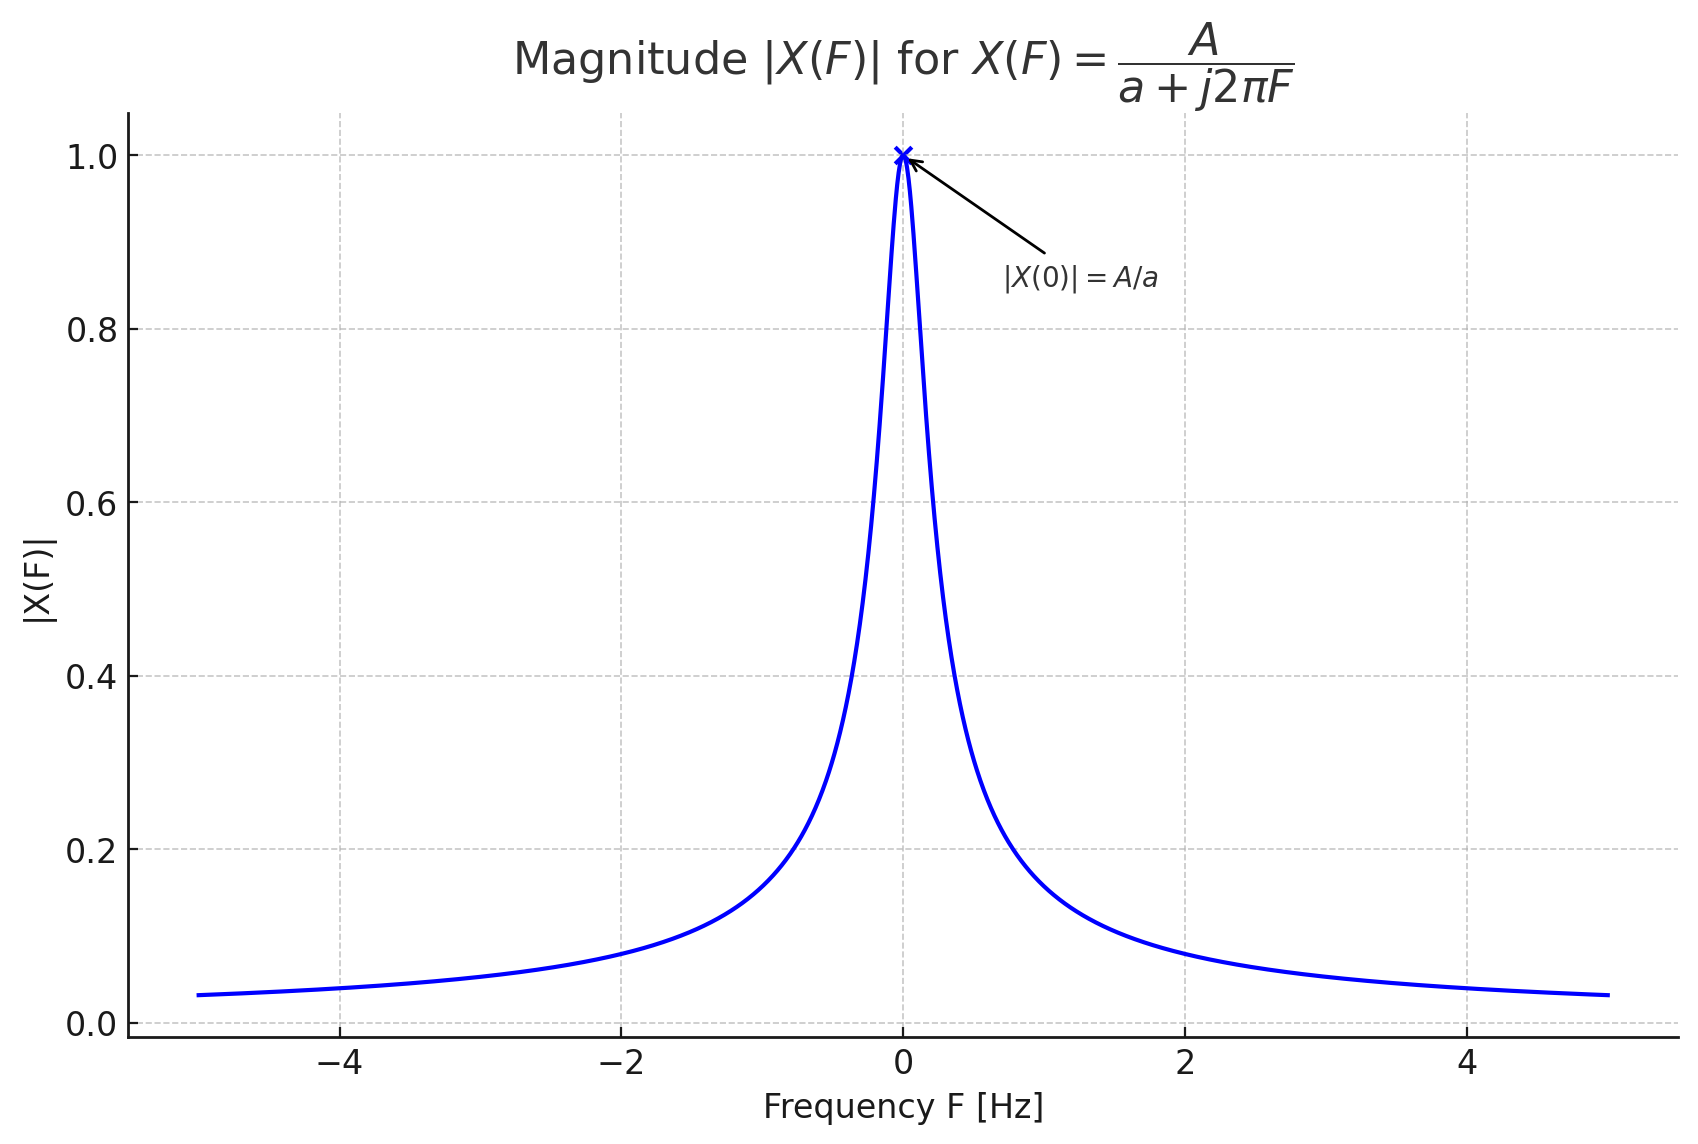
\includegraphics[width=1\linewidth]{Auxiliar_3_2} % <-- pon la extensión si hace falta
    \caption{Magnitud $|X(\omega)|$ para $X(\omega)=\frac{A}{a+j\omega}$. Se observa un máximo en $\omega=0$ igual a $A/a$, y la magnitud decae rápidamente para frecuencias altas, mostrando el comportamiento típico de un filtro pasabajo exponencial.}
    \label{fig:mag_XF1}
  \end{subfigure}
  \hfill
  \begin{subfigure}[t]{0.48\textwidth}
    \centering
    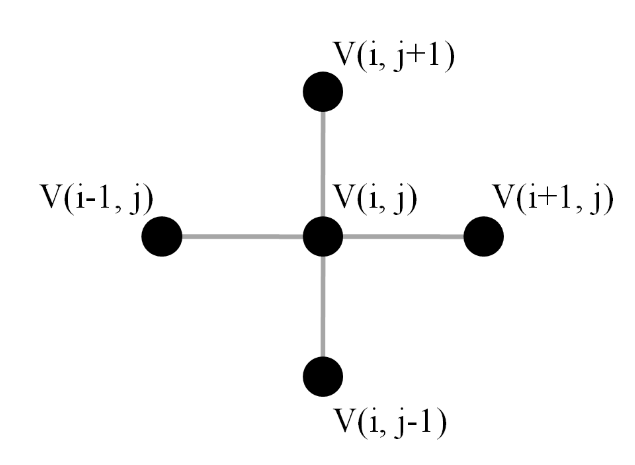
\includegraphics[width=1\linewidth]{Auxiliar_3_3}
    \caption{Fase $\measuredangle X(\omega)$ para $X(\omega)=\frac{A}{a+j\omega}$. La fase parte en $0$ para $\omega=0$ y varía suavemente desde $+\pi/2$ a $-\pi/2$ al aumentar $|\omega|$, indicando el retardo de fase introducido por el sistema.}
    \label{fig:fase_XF}
  \end{subfigure}

  \caption{Magnitud y fase de la transformada de Fourier para $x(t)=A e^{-a t}u(t)$. La magnitud tiene máximo en $\omega=0$ y la fase varía de $+\pi/2$ a $-\pi/2$ según la frecuencia, mostrando el efecto de la exponencial sobre el espectro.}
  \label{fig:mag_fase_XF}
\end{figure}


Sea ahora la siguiente función:
\begin{equation}
x(t)=A\,e^{-a|t|},\qquad a>0,
\end{equation}
que es par. Separando para \(t\ge 0\) y \(t<0\),
\begin{align}
X(\omega)
 &= \int_{-\infty}^{\infty} A e^{-a|t|} e^{-j\omega t}\,dt \\
 &= \int_{-\infty}^{0} A e^{+a t} e^{-j\omega t}\,dt
   + \int_{0}^{\infty} A e^{-a t} e^{-j\omega t}\,dt \\
 &= A\int_{-\infty}^{0} e^{(a-j\omega)t}\,dt
   +A\int_{0}^{\infty} e^{-(a+j\omega)t}\,dt \\
 &= A\left[\frac{1}{a-j\omega}e^{(a-j\omega)t}\right]_{-\infty}^{0}
   +A\left[\frac{-1}{a+j\omega}e^{-(a+j\omega)t}\right]_{0}^{\infty} \\
 &= \frac{A}{a-j\omega}+\frac{A}{a+j\omega}
  = \frac{A\big((a+j\omega)+(a-j\omega)\big)}{a^{2}+\omega^{2}} \\
 &= \frac{2A a}{a^{2}+\omega^{2}}.
\end{align}

Como \(x(t)\) es par, \(X(\omega)\) es real y par:
\begin{align}
|X(\omega)|
  &= \frac{2A a}{a^{2}+\omega^{2}},\\
\angle X(\omega)
  &= 0\quad \text{(para todo \(\omega\), salvo el signo en \(\omega\) donde \(X(\omega)>0\))}.
\end{align}
Luego gráficamente tenemos lo siguiente:
\begin{figure}[H]
  \centering

  \begin{subfigure}[t]{0.48\textwidth}
    \centering
    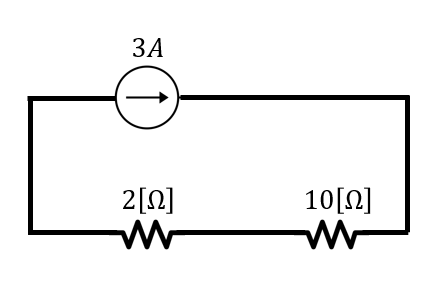
\includegraphics[width=1\linewidth]{Auxiliar_3_4} % <-- pon la extensión si hace falta
    \caption{Magnitud $|X(\omega)|$ para $X(\omega)=\frac{2Aa}{a^2+\omega^2}$. Se observa un máximo en $\omega=0$ igual a $2A/a$, y la magnitud es real, par y decae para frecuencias altas, mostrando el espectro de una exponencial simétrica.}
    \label{fig:mag_XF2}
  \end{subfigure}
  \hfill
  \begin{subfigure}[t]{0.48\textwidth}
    \centering
    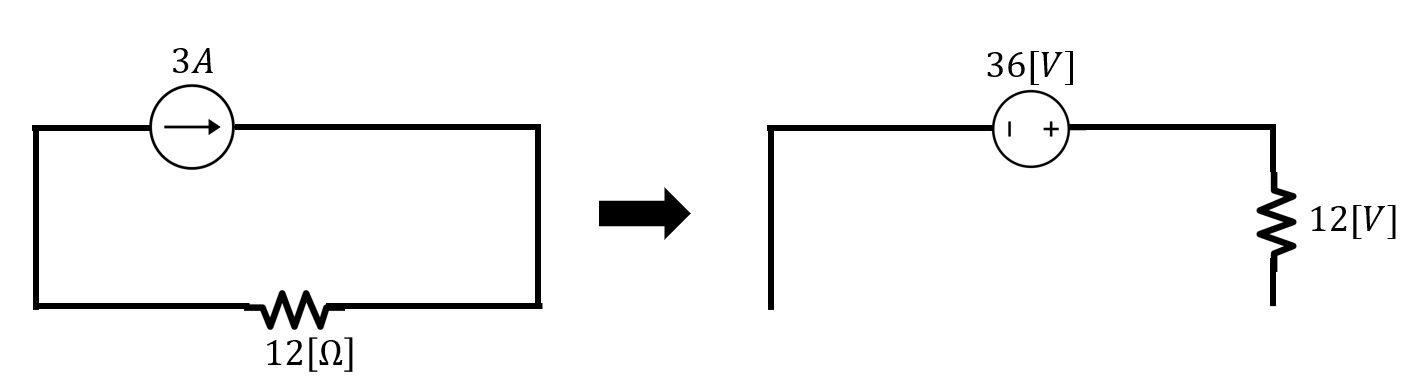
\includegraphics[width=1\linewidth]{Auxiliar_3_5}
    \caption{Fase $\measuredangle X(\omega)$ para $X(\omega)=\frac{2Aa}{a^2+\omega^2}$. La fase es cero para todo $\omega$, lo que indica que la señal original es par y su transformada es completamente real.}
    \label{fig:fase_XF2}
  \end{subfigure}

  \caption{Magnitud y fase de la transformada de Fourier para $x(t)=A e^{-a|t|}$. La magnitud es real y par, con máximo en $\omega=0$, y la fase es cero en todo el dominio de frecuencias.}
  \label{fig:mag_fase_XF2}
\end{figure}

\subsection*{Resolución 3.2}
Los coeficientes de la serie de Fourier \( \{c_k\}_{k\in\mathbb{Z}} \) permiten expresar una señal periódica como combinación lineal de sinusoides complejas. En la forma compleja,
\begin{equation}
x(t)=\sum_{k=-\infty}^{\infty} c_k\,e^{jk\omega_0 t}, 
\qquad \omega_0=\frac{2\pi}{T_0},
\end{equation}
donde \(T_0\) es el período fundamental. Los coeficientes se obtienen (sobre cualquier intervalo de longitud \(T_0\)) como
\begin{equation}
c_k=\frac{1}{T_0}\int_{t_0}^{t_0+T_0} x(t)\,e^{-jk\omega_0 t}\,dt .
\end{equation}
Para convertir senos y cosenos a exponenciales usamos las identidades de Euler:
\begin{align}
\cos(\theta) &= \frac{e^{j\theta}+e^{-j\theta}}{2}, &
\sin(\theta) &= \frac{e^{j\theta}-e^{-j\theta}}{2j}.
\end{align}

Dada la señal
\begin{equation}
x(t)=1+\sin(\omega_0 t)+2\cos(\omega_0 t)+\cos\!\left(2\omega_0 t+\frac{\pi}{4}\right),
\end{equation}
la escribimos en forma exponencial y agrupamos por armónicos \(e^{jk\omega_0 t}\):
\begin{align}
x(t)
&= 1
+ \frac{1}{2j}e^{j\omega_0 t}-\frac{1}{2j}e^{-j\omega_0 t}
+ \left(e^{j\omega_0 t}+e^{-j\omega_0 t}\right)
+ \frac{1}{2}e^{j\frac{\pi}{4}}e^{j2\omega_0 t}
+ \frac{1}{2}e^{-j\frac{\pi}{4}}e^{-j2\omega_0 t} \\
&= 1
+ \Big(1+\tfrac{1}{2j}\Big)e^{j\omega_0 t}
+ \Big(1-\tfrac{1}{2j}\Big)e^{-j\omega_0 t}
+ \frac{1}{2}e^{j\frac{\pi}{4}}e^{j2\omega_0 t}
+ \frac{1}{2}e^{-j\frac{\pi}{4}}e^{-j2\omega_0 t}.
\end{align}
Identificando término a término con \(x(t)=\sum_k c_k e^{jk\omega_0 t}\), los coeficientes complejos son:
\begin{align}
c_0 &= 1, \\
c_{1} &= 1+\frac{1}{2j}=1-\frac{j}{2}, \\
c_{-1} &= 1-\frac{1}{2j}=1+\frac{j}{2}, \\
c_{2} &= \frac{1}{2}e^{j\frac{\pi}{4}}=\frac{\sqrt{2}}{4}(1+j), \\
c_{-2} &= \frac{1}{2}e^{-j\frac{\pi}{4}}=\frac{\sqrt{2}}{4}(1-j), \\
c_k &= 0 \quad \text{para } |k|\ge 3.
\end{align}
Obsérvese que, al ser \(x(t)\) real, se cumple la simetría conjugada \(c_{-k}=c_k^{*}\).


\end{solution}
%----------------------------
\question Encuentre la transformada de Fourier de cada una de las siguientes señales y dibuje la magnitud y la fase como función de la frecuencia, incluyendo tanto frecuencias positivas como negativas.

\begin{enumerate}
    \item $\delta(t - 5)$
    \item $e^{(-1+j2)t}u(t)$
\end{enumerate}
%----------------------------
\begin{solution}
\subsection*{Resolucion 3.1}
Se busca obtener por lo tanto utilizaremos:
\begin{align}
  X(\omega) &= \int_{-\infty}^{\infty} x(t)\,e^{-j\omega t}\,dt
\end{align}
Luego tenemos que:
\begin{itemize}
  \item \textbf{Caso 1:} \(x(t)=\delta(t-5)\)
  Tenemos por lo tanto:
  \begin{align}
    X(\omega) &= \int_{-\infty}^{\infty} \delta(t-5)\,e^{-j\omega t}\,dt \\
         &= e^{-j\omega \cdot 5} \\
         &= e^{-j5\omega}
  \end{align}
  Luego la magnitud y fase vienen dadas por:
  \begin{align}
    |X(\omega)| &= 1, \\
    \measuredangle X(\omega) &= -5\omega
  \end{align}
  \begin{figure}[H]
\centering
\begin{tikzpicture}
\begin{groupplot}[
  group style={group size=2 by 1, horizontal sep=2.5cm},
  width=7cm, height=6cm,
  axis lines=middle,
  xmin=-10, xmax=10,
  tick style={thick},
  xlabel style={at={(axis description cs:0.5,-0.08)}},
  ylabel style={at={(axis description cs:-0.1,0.5)}},
  title style={at={(axis description cs:0.5,1.05)}}
]

% --- Magnitud |X(w)| = 1 ---
\nextgroupplot[
  ymin=0, ymax=1.2,
  xtick={-10,-5,0,5,10},
  ytick={0,1},
  xlabel={$\,\omega$},
  ylabel={$|X(\omega)|$},
  title={Magnitud}
]
\addplot[domain=-10:10, samples=2, very thick] {1};

% --- Fase ∠X(w) = -5 w ---
\nextgroupplot[
  ymin=-55, ymax=55,
  xtick={-10,-5,0,5,10},
  ytick={-50,-25,0,25,50},
  xlabel={$\,\omega$},
  ylabel={$\measuredangle X(\omega)$ (rad)},
  title={Fase}
]
\addplot[domain=-10:10, samples=2, very thick] {-5*x};

\end{groupplot}
\end{tikzpicture}
\caption{Gráficas de $X(\omega)=e^{-j5\omega}$: $|X(\omega)|=1$ y $\measuredangle X(\omega)=-5\omega$.}
\end{figure}

  \item \textbf{Caso 2:} \(x(t)=e^{(-1+j2)t}u(t)\)
  Tenemos por lo tanto:
  \begin{align}
    X(\omega) &= \int_{-\infty}^{\infty} e^{(-1+j2)t}u(t)\,e^{-j\omega t}\,dt \\
         &= \int_{0}^{\infty} e^{(-1+j2-j\omega)t}\,dt \\
         &= \left[\frac{-1}{-1+j2-j\omega}e^{(-1+j2-j\omega)t}\right]_{0}^{\infty} \\
         &= \frac{1}{1-j(2-\omega)}
  \end{align}
  Luego la magnitud y fase vienen dadas por:
  \begin{align}
    |X(\omega)| &= \frac{1}{\sqrt{1+(2-\omega)^{2}}}, \\
    \measuredangle X(\omega) &= \arctan(2-\omega)
  \end{align}
\begin{figure}[H]
\centering
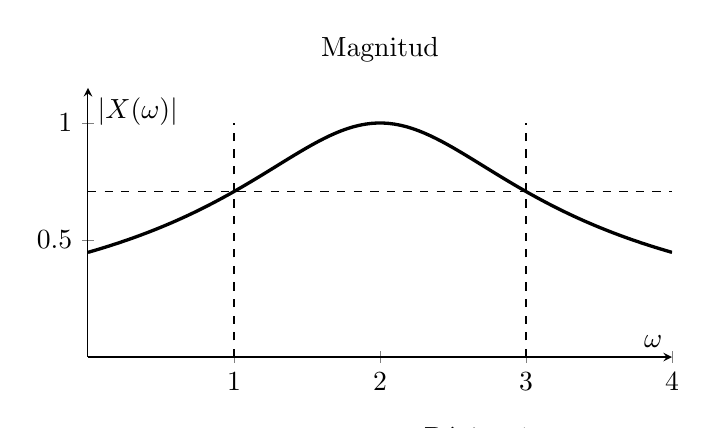
\begin{tikzpicture}
\begin{axis}[
  width=9cm, height=5cm,
  axis lines=middle,
  xmin=0, xmax=4,
  ymin=0, ymax=1.15,
  xtick={0,1,2,3,4},
  ytick={0,0.5,1},
  xlabel={$\,\omega$},
  ylabel={$|X(\omega)|$},
  title={Magnitud}
]
\addplot[very thick, domain=0:4, samples=100] {1/sqrt(1 + (x-2)^2)};
% Marcas en 1/sqrt(2) y en ω=1,3 (ancho a -3 dB)
\addplot[dashed] coordinates {(0,0.707) (4,0.707)};
\addplot[dashed] coordinates {(1,0) (1,1)};
\addplot[dashed] coordinates {(3,0) (3,1)};
\end{axis}
\end{tikzpicture}
\caption{Magnitud: Para $x(t)=e^{(-1+j2)t}u(t)$, se obtiene $|X(\omega)|=\frac{1}{\sqrt{1+(\omega-2)^2}}$.}
\end{figure}

\begin{figure}[H]
\centering
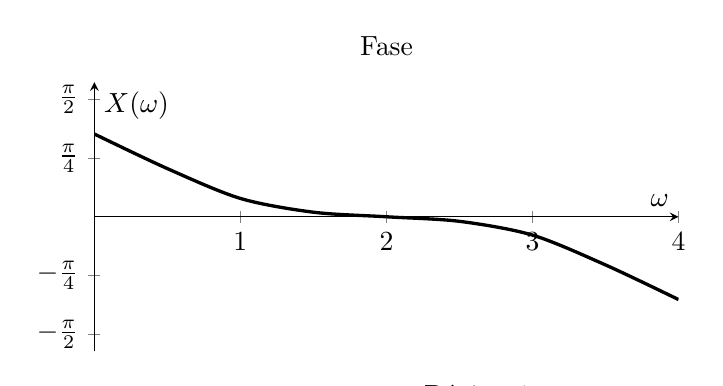
\begin{tikzpicture}
\begin{axis}[
  width=9cm, height=5cm,
  axis lines=middle,
  xmin=0, xmax=4,
  ymin=-1.8, ymax=1.8,
  xtick={0,1,2,3,4},
  ytick={-1.5708,-0.7854,0,0.7854,1.5708},
  yticklabels={$-\frac{\pi}{2}$,$-\frac{\pi}{4}$,$0$,$\frac{\pi}{4}$,$\frac{\pi}{2}$},
  xlabel={$\,\omega$},
  ylabel={$\measuredangle X(\omega)$},
  title={Fase}
]
\addplot[very thick, smooth] coordinates {
  (0,1.107) (0.5,0.644) (1,0.245) (1.5,0.061) (2,0) 
  (2.5,-0.061) (3,-0.245) (3.5,-0.644) (4,-1.107)
};
\end{axis}
\end{tikzpicture}
\caption{Fase: Para $x(t)=e^{(-1+j2)t}u(t)$, se obtiene $\measuredangle X(\omega)=-\tan^{-1}(\omega-2)$.}
\end{figure}

\end{itemize}
\end{solution}
%---------------------------
\question En este problema exploramos la definición de la transformada de Fourier de una señal periódica.

\begin{enumerate}
    \item Demuestre que si $x_3(t) = ax_1(t) + bx_2(t)$, entonces $X_3(\omega) = aX_1(\omega) + bX_2(\omega)$.
    
    \item Verifique que
    \begin{equation}
        e^{j\omega_0 t} = \frac{1}{2\pi} \int_{-\infty}^{\infty} 2\pi\delta(\omega - \omega_0)e^{j\omega t} d\omega
    \end{equation}
    A partir de esta observación, argumente que la transformada de Fourier de $e^{j\omega_0 t}$ es $2\pi\delta(\omega - \omega_0)$.
    
    \item Recuerde la ecuación de síntesis para la serie de Fourier:
    \begin{equation}
        x(t) = \sum_{k=-\infty}^{\infty} a_k e^{jk(2\pi/T)t}
    \end{equation}
    
    Tomando la transformada de Fourier de ambos lados y usando los resultados de las partes (a) y (b), demuestre que
    \begin{equation}
        X(\omega) = \sum_{k=-\infty}^{\infty} 2\pi a_k \delta\left(\omega - \frac{2\pi k}{T}\right)
    \end{equation}
    
    \item Dibuje $X(\omega)$ para su respuesta al Problema P8.1(d) para $|\omega| \leq 4\pi/T_0$.
\end{enumerate}
%----------------------------
\begin{solution}
\subsection*{Resolución 4.1}

\textbf{(a)} Para demostrar la propiedad de linealidad de la transformada de Fourier:

Por definición, la transformada de Fourier es:
\begin{equation}
X_3(\omega) = \int_{-\infty}^{\infty} x_3(t)e^{-j\omega t} dt
\end{equation}

Sustituyendo $x_3(t) = ax_1(t) + bx_2(t)$:
\begin{align}
X_3(\omega) &= \int_{-\infty}^{\infty} [ax_1(t) + bx_2(t)]e^{-j\omega t} dt \\
&= \int_{-\infty}^{\infty} ax_1(t)e^{-j\omega t} dt + \int_{-\infty}^{\infty} bx_2(t)e^{-j\omega t} dt \\
&= a \int_{-\infty}^{\infty} x_1(t)e^{-j\omega t} dt + b \int_{-\infty}^{\infty} x_2(t)e^{-j\omega t} dt = aX_1(\omega) + bX_2(\omega)
\end{align}

\subsection*{Resolución 4.2}

\textbf{(b)} Recordemos la propiedad de tamizado (sifting) de la función impulso unitario:
\begin{equation}
\int_{-\infty}^{\infty} h(t)\delta(t - t_0) dt = h(t_0)
\end{equation}

Por lo tanto:
\begin{equation}
\int_{-\infty}^{\infty} 2\pi\delta(\omega - \omega_0)e^{j\omega t} d\omega = 2\pi e^{j\omega_0 t}
\end{equation}

Así:
\begin{equation}
\frac{1}{2\pi} \int_{-\infty}^{\infty} 2\pi\delta(\omega - \omega_0)e^{j\omega t} d\omega = e^{j\omega_0 t}
\end{equation}

Nótese que la integral que relaciona $2\pi\delta(\omega - \omega_0)$ y $e^{j\omega_0 t}$ es exactamente de la forma:
\begin{equation}
x(t) = \frac{1}{2\pi} \int_{-\infty}^{\infty} X(\omega)e^{j\omega t} d\omega,
\end{equation}

donde $x(t) = e^{j\omega_0 t}$ y $X(\omega) = 2\pi\delta(\omega - \omega_0)$. Así, podemos pensar en $e^{j\omega_0 t}$ como la transformada inversa de Fourier de $2\pi\delta(\omega - \omega_0)$. Por lo tanto, $2\pi\delta(\omega - \omega_0)$ es la transformada de Fourier de $e^{j\omega_0 t}$.

\textbf{(c)} Usando el resultado de la parte (a), tenemos:

\begin{equation}
X(\omega) = \mathcal{F}\{x(t)\} = \mathcal{F}\left\{ \sum_{k=-\infty}^{\infty} a_k e^{jk(2\pi/T)t} \right\} = \sum_{k=-\infty}^{\infty} a_k \mathcal{F}\{e^{jk(2\pi/T)t}\}
\end{equation}

De la parte (b):
\begin{equation}
\mathcal{F}\{e^{jk(2\pi/T)t}\} = 2\pi\delta\left(\omega - \frac{2\pi k}{T}\right)
\end{equation}

Por lo tanto:
\begin{equation}
X(\omega) = \sum_{k=-\infty}^{\infty} 2\pi a_k \delta\left(\omega - \frac{2\pi k}{T}\right)
\end{equation}
\subsection*{Resolución 4.4}
Se busca graficar \(X(\omega)\) para la respuesta del problema en el rango \(|\omega| \leq 4\pi/T_0\), con lo que tenemos que:
\begin{figure}[H]
\centering
\begin{tikzpicture}[x=2.4cm,y=1.4cm,>=Latex]
  % Eje ω
  \draw[thick] (-2.4,0) -- (2.4,0) node[below right] {$\omega$};

  % Título arriba
  \node at (0,2.2) {$\tilde X(\omega)$};

  % ----- parámetros de alturas (solo estéticos) -----
  \def\Aup{1.4}     % altura impulso central (4π/3)
  \def\Bup{1.1}     % altura impulsos laterales positivos (2 sin(2π/3))
  \def\Bdn{0.8}     % magnitud impulsos laterales negativos (sin(4π/3))

  % ----- impulsos: posiciones aproximadas -----
  % izquierda: negativo (sin 4π/3) y positivo (2 sin 2π/3)
  \draw[very thick,-{Latex}] (-1.60,0) -- (-1.60,-\Bdn);
  \node[below] at (-1.60,-\Bdn) {$\displaystyle \sin\!\frac{4\pi}{3}$};

  \draw[very thick,-{Latex}] (-0.85,0) -- (-0.85,\Bup);
  \node[above] at (-0.85,\Bup) {$\displaystyle 2\sin\!\frac{2\pi}{3}$};

  % centro: impulso grande (4π/3)
  \draw[very thick,-{Latex}] (0,0) -- (0,\Aup);
  \node[above] at (0,\Aup) {$\displaystyle \frac{4\pi}{3}$};

  % derecha: positivo (2 sin 2π/3) y negativo (sin 4π/3)
  \draw[very thick,-{Latex}] (0.85,0) -- (0.85,\Bup);
  \node[above] at (0.85,\Bup) {$\displaystyle 2\sin\!\frac{2\pi}{3}$};

  \draw[very thick,-{Latex}] (1.60,0) -- (1.60,-\Bdn);
  \node[below] at (1.60,-\Bdn) {$\displaystyle \sin\!\frac{4\pi}{3}$};

  % marca textual bajo el impulso a la derecha del centro
  \draw (0.85,0.03) -- (0.85,-0.03);
  \node[below] at (0.85,-0.08) {$\displaystyle \frac{2\pi}{T_0}$};
\end{tikzpicture}
\caption{Espectro discreto con impulsos (flechas) y amplitudes rotuladas.}
\end{figure}

\end{solution}
%----------------------------
\question Encuentre la señal $x[n]$ si su transformada de Fourier a tiempo discreto está dada por

%----------------------------
\begin{figure}[H]
\centering
\begin{tikzpicture}[>=latex, line cap=round]

% ===== Parámetros editables =====
\def\wc{2.2}   % posición de ±\omega_c sobre el eje x
\def\halfW{0.4}% mitad del ancho de banda (W/2)
\def\H{2.0}    % altura de los rectángulos (amplitud)
% =================================

% Ejes
\draw[->] (-5,0) -- (5.5,0) node[below] {$\omega$};
\draw[->] (0,-0.2) -- (0,3) node[left] {$X(\omega)$};

% Marcas y etiquetas en x
\draw (-3.8,0.08) -- (-3.8,-0.08) node[below=2pt] {$-\pi$};
\draw ( 3.8,0.08) -- ( 3.8,-0.08) node[below=2pt] {$\pi$};
\draw (-\wc,0.08) -- (-\wc,-0.08) node[below=2pt] {$-\omega_c$};
\draw ( \wc,0.08) -- ( \wc,-0.08) node[below=2pt] {$\omega_c$};

% Marcas y etiquetas en y
\draw ( 0.08,1) -- (-0.08,1) node[left=2pt]  {$1$};
\draw ( 0.08,2) -- (-0.08,2) node[left=2pt]  {$2$};

% Rectángulo banda izquierda (centrado en -\omega_c)
\draw[line width=1.0pt]
  (-\wc-\halfW,0) -- (-\wc-\halfW,\H) -- (-\wc+\halfW,\H) -- (-\wc+\halfW,0);

% Rectángulo banda derecha (centrado en +\omega_c)
\draw[line width=1.0pt]
  (\wc-\halfW,0) -- (\wc-\halfW,\H) -- (\wc+\halfW,\H) -- (\wc+\halfW,0);

% Llave que indica el ancho W sobre la banda derecha
\draw[decorate, decoration={brace, amplitude=4pt}]
  (\wc-\halfW,\H+0.3) -- (\wc+\halfW,\H+0.3)
  node[midway, above=6pt] {$W$};

\end{tikzpicture}
\caption{Transformada de Fourier a tiempo discreto $X(\omega)$ de la señal $x[n]$.}
\end{figure}
Ahora considere una transformada de Fourier que en el rango $\left] -\frac{\pi}{2}, \frac{\pi}{2} \right]$ viene dado por:
\begin{align}
  X(\omega)= -\omega^{2} + \frac{\pi^{2}}{4}
\end{align}
bosqueje esta transformada y obtenga la señal en tiempo discreto asociada.
%----------------------------
\begin{solution}

\subsection*{Resolución 5.1}
 Para encontrar la señal $x[n]$ a partir de su transformada de Fourier a tiempo discreto $X(\omega)$, utilizamos la transformada inversa. Este procedimiento consiste en aplicar la integral inversa de la DTFT, que permite reconstruir la señal en el dominio temporal a partir de su representación espectral. A continuación, se presenta el planteamiento general, luego la DTFT inversa es
\[
x[n]=\frac{1}{2\pi}\int_{-\pi}^{\pi}X(\omega)\,e^{j\omega n}\,d\omega.
\]
Del gráfico, $X(\omega)=2$ sólo en los intervalos
\[
\left[-\omega_c-\frac{W}{2},\, -\omega_c+\frac{W}{2}\right]
\quad\text{y}\quad
\left[\omega_c-\frac{W}{2},\, \omega_c+\frac{W}{2}\right],
\]
y $X(\omega)=0$ fuera de ellos. Por lo tanto,
\begin{align*}
x[n]
&=\frac{1}{2\pi}\int_{-\omega_c-\frac{W}{2}}^{-\omega_c+\frac{W}{2}}2\,e^{j\omega n}\,d\omega
+\frac{1}{2\pi}\int_{\omega_c-\frac{W}{2}}^{\omega_c+\frac{W}{2}}2\,e^{j\omega n}\,d\omega. \tag{$\star$}\label{star}
\end{align*}
Luego analizaremos dos casos de interes: $n\neq 0$ y $n=0$.
\begin{itemize}
  \item  \textbf{Cálculo para $n\neq 0$.} Cada integral es elemental:
\[
\int e^{j\omega n}\,d\omega=\frac{e^{j\omega n}}{j n}.
\]
Aplicando a \eqref{star}:
\begin{align*}
x[n]
&=\frac{1}{\pi}\left[\frac{e^{j\omega n}}{j n}\right]_{-\omega_c-\frac{W}{2}}^{-\omega_c+\frac{W}{2}}
+\frac{1}{\pi}\left[\frac{e^{j\omega n}}{j n}\right]_{\omega_c-\frac{W}{2}}^{\omega_c+\frac{W}{2}}\\[2mm]
&=\frac{1}{\pi j n}\Big(
e^{j n(-\omega_c+\frac{W}{2})}-e^{j n(-\omega_c-\frac{W}{2})}
+e^{j n(\omega_c+\frac{W}{2})}-e^{j n(\omega_c-\frac{W}{2})}
\Big)\\[1mm]
&=\frac{1}{\pi j n}\Big(
e^{-j n\omega_c}\big(e^{j n\frac{W}{2}}-e^{-j n\frac{W}{2}}\big)
+e^{+j n\omega_c}\big(e^{j n\frac{W}{2}}-e^{-j n\frac{W}{2}}\big)
\Big)\\[1mm]
&=\frac{1}{\pi j n}\,\underbrace{\big(e^{j n\frac{W}{2}}-e^{-j n\frac{W}{2}}\big)}_{=\,2j\sin(\frac{nW}{2})}\,
\underbrace{\big(e^{j n\omega_c}+e^{-j n\omega_c}\big)}_{=\,2\cos(n\omega_c)}\\[1mm]
&=\boxed{\,x[n]=\dfrac{4}{\pi n}\,\sin\!\Big(\frac{nW}{2}\Big)\cos(n\omega_c)\,},\qquad n\neq 0.
\end{align*}
Donde se han utilizado las identidades de euler y la definición de la función seno y coseno en términos de exponenciales complejas, las cuales son:
\begin{align}
\sin(x)&=\frac{e^{jx}-e^{-jx}}{2j},\\
\cos(x)&=\frac{e^{jx}+e^{-jx}}{2}.
\end{align}
\item \textbf{Caso $n=0$.} Usando directamente el área del espectro:
\[
\begin{aligned}
  x(0) &= \frac{1}{2\pi} \int_{-\omega_c-\frac{W}{2}}^{-\omega_c+\frac{W}{2}} 2\,d\omega
         + \frac{1}{2\pi} \int_{\omega_c-\frac{W}{2}}^{\omega_c+\frac{W}{2}} 2\,d\omega \\
       &= \frac{1}{2\pi} \left[ 2 \cdot \left( \left(-\omega_c+\frac{W}{2}\right) - \left(-\omega_c-\frac{W}{2}\right) \right)
         + 2 \cdot \left( \left(\omega_c+\frac{W}{2}\right) - \left(\omega_c-\frac{W}{2}\right) \right) \right] \\
       &= \frac{1}{2\pi} \left[ 2 \cdot (W) + 2 \cdot (W) \right] \\
       &= \frac{1}{2\pi} (4W) \\
       &= \frac{2W}{\pi}
\end{aligned}
\]
Es decir, $x[0]$ corresponde al área total bajo el espectro $X(\omega)$, que es la suma de las áreas de los dos rectángulos de altura $2$ y ancho $W$ cada uno.
\end{itemize}
Con lo que finalmente se tendra la funcion discreta sera:
\[
x[n]=
\begin{cases}
\dfrac{4}{\pi n}\,\sin\!\big(\frac{nW}{2}\big)\cos(n\omega_c), & n\neq 0,\\[2mm]
\dfrac{2W}{\pi}, & n=0.
\end{cases}
\]
% Requiere: \usepackage{tikz, pgfplots} en el preámbulo
% y (opcional) \pgfplotsset{compat=1.18}
\begin{figure}[H]
\centering
\begin{tikzpicture}
\pgfplotsset{compat=1.18}
% ==== Parámetros (en radianes) ====
\pgfmathsetmacro{\W}{1.2}      % ancho de banda W
\pgfmathsetmacro{\wc}{0.6}     % frecuencia central \omega_c
\pgfmathtruncatemacro{\N}{30}  % |n| máximo a graficar

\begin{axis}[
    width=18cm,height=6.5cm,
    axis lines=middle,
    xlabel={$n$}, ylabel={$x[n]$},
    xmin=-\N-1, xmax=\N+1,
    ymajorgrids,
    legend style={at={(0.02,0.98)},anchor=north west,draw=none,fill=none},
    tick align=outside
]

% === Stems discretos ===
% Usamos un foreach para evaluar exactamente en n enteros
\pgfplotsinvokeforeach{-\N,...,\N}{
  \addplot+[ycomb,mark=*,thick]
  coordinates {
    (#1, { (#1==0) ? (2*\W/pi) : ( 4/(pi*(#1)) * sin(deg((#1)*\W/2)) * cos(deg((#1)*\wc)) ) })
  };
}

% Leyenda movida más a la izquierda para mejor visibilidad
\node[anchor=north east] at (axis cs:-5,0.6) {$\displaystyle x[n]=\begin{cases}\frac{4}{\pi n}\sin\!\big(\frac{nW}{2}\big)\cos(n\omega_c),& n\neq0\\[3pt]\frac{2W}{\pi},& n=0\end{cases}$};

% Punto en n=0 resaltado y etiqueta opcional
\addplot+[only marks, mark=*, mark size=2.3pt]
coordinates {(0, {2*\W/pi})};
\node[anchor=south east] at (axis cs:0,{2*\W/pi}) {$\;\;x[0]=\tfrac{2W}{\pi}$};

\end{axis}
\end{tikzpicture}
\caption{Gráfico tipo stem de $x[n]$ para $W=1.2$ rad y $\omega_c=2.2$ rad.}
\label{fig:xn_stem}
\end{figure}

\subsection*{Resolución 5.2}
Tenemos que la transformada de Fourier a tiempo discreto es
\[
X(\omega)=
\begin{cases}
-\omega^2+\dfrac{\pi^2}{4}, & \omega\in\left[-\dfrac{\pi}{2},\,\dfrac{\pi}{2}\right],\\[2mm]
0, & \text{en otro caso}.
\end{cases}
\]
Luego graficamente se tiene que:
\begin{figure}[H]
\centering
\begin{tikzpicture}[scale=1.2]

% Ejes
\draw[->] (-3.5,0) -- (3.5,0) node[right] {$\omega$};
\draw[->] (0,0) -- (0,4) node[above] {$X(\omega)$};

% Curva parabólica X(w) = -w^2 + pi^2/4 en [-pi/2, pi/2]
\draw[thick,domain=-1.57:1.57,samples=100] 
  plot(\x,{-(\x)^2 + pi^2/4});

% Línea discontinua en pi^2/4
\draw[dashed] (-0.3,{pi^2/4}) -- (0.3,{pi^2/4});
\node[right] at (0.3,{pi^2/4}) {$\tfrac{\pi^2}{4}$};

% Marcas en los ejes
\draw (-3.14,0.1) -- (-3.14,-0.1) node[below] {$-\pi$};
\draw (-1.57,0.1) -- (-1.57,-0.1) node[below] {$-\tfrac{\pi}{2}$};
\draw ( 1.57,0.1) -- ( 1.57,-0.1) node[below] {$\tfrac{\pi}{2}$};
\draw ( 3.14,0.1) -- ( 3.14,-0.1) node[below] {$\pi$};

\end{tikzpicture}
\caption{Espectro $X(\omega)=-\omega^2+\tfrac{\pi^2}{4}$ en $[-\pi/2,\pi/2]$.}
\end{figure}
Por definición de la DTFT inversa, tenemos que:
\begin{align}
  x[n]= \frac{1}{2\pi}\int_{-\pi}^{\pi}X(\omega)\,e^{j\omega n}\,d\omega.
\end{align}
Luego tenemos que la inversa de la DTFT para nuestro caso será:
\begin{align}
x[n]&=\frac{1}{2\pi}\int_{-\frac{\pi}{2}}^{\frac{\pi}{2}}\Big(-\omega^2+\frac{\pi^2}{4}\Big)e^{j\omega n}\,d\omega\\
&=\frac{1}{2\pi}\Big[\,\underbrace{-\!\int_{-\frac{\pi}{2}}^{\frac{\pi}{2}}\omega^2 e^{j\omega n}\,d\omega}_{(I)}\;
+\;\underbrace{\frac{\pi^2}{4}\!\int_{-\frac{\pi}{2}}^{\frac{\pi}{2}} e^{j\omega n}\,d\omega}_{(II)}\,\Big].
\end{align}
Comenzamos calculando el termino $(II)$. para $n\neq 0$, con lo que obtenemos que:
\begin{align*}
(II)&=\frac{\pi^2}{4}\left[\frac{e^{j\omega n}}{j n}\right]_{-\frac{\pi}{2}}^{\frac{\pi}{2}}
=\frac{\pi^2}{4}\cdot\frac{e^{j n\frac{\pi}{2}}-e^{-j n\frac{\pi}{2}}}{j n}
=\frac{\pi^2}{2n}\,\sin\!\Big(\frac{n\pi}{2}\Big).
\end{align*}
Por otro lado para el termino $(I)$, tenemos que hacer integración por partes. Primera integración por partes con $u=\omega^2$, $dv=e^{j\omega n}\,d\omega$:
\[
\int \omega^2 e^{j\omega n}d\omega=\frac{\omega^2 e^{j\omega n}}{j n}-\int \frac{2\omega e^{j\omega n}}{j n}\,d\omega.
\]
Donde:
\begin{itemize}
  \item $u=\omega^2 \implies du=2\omega d\omega$
  \item $dv=e^{j\omega n}d\omega \implies v=\frac{e^{j\omega n}}{j n}$
\end{itemize}
Por la fórmula de integración por partes $\int u\,dv = uv - \int v\,du$.La segunda integración por partes en $\displaystyle \int \omega e^{j\omega n}d\omega$ con $u=\omega$, $dv=e^{j\omega n}d\omega$:
\[
\int \omega e^{j\omega n}d\omega=\frac{\omega e^{j\omega n}}{j n}-\int \frac{e^{j\omega n}}{j n}\,d\omega
\]
Donde:
\begin{itemize}
  \item $u=\omega \implies du=d\omega$
  \item $dv=e^{j\omega n}d\omega \implies v=\frac{e^{j\omega n}}{j n}$
\end{itemize}
Aplicando integración por partes:
\[
\int \omega e^{j\omega n}d\omega = \omega \cdot \frac{e^{j\omega n}}{j n} - \int \frac{e^{j\omega n}}{j n} d\omega = \frac{\omega e^{j\omega n}}{j n} - \frac{1}{j n} \int e^{j\omega n} d\omega
\]
Pero $\int e^{j\omega n} d\omega = \frac{e^{j\omega n}}{j n}$, así que:
\[
\int \omega e^{j\omega n}d\omega = \frac{\omega e^{j\omega n}}{j n} - \frac{e^{j\omega n}}{(j n)^2}
\]
Sustituyendo, obtenemos la primitiva cerrada:
\[
\int \omega^2 e^{j\omega n}d\omega
=\frac{\omega^2 e^{j\omega n}}{j n}-\frac{2\omega e^{j\omega n}}{(j n)^2}
+\frac{2 e^{j\omega n}}{(j n)^3}+C.
\]
Sustituyendo el resultado anterior en la primera integración por partes:
\[
\int \omega^2 e^{j\omega n}d\omega = \frac{\omega^2 e^{j\omega n}}{j n} - \frac{2}{j n} \left( \frac{\omega e^{j\omega n}}{j n} - \frac{e^{j\omega n}}{(j n)^2} \right )
\]
Desarrollando los términos:
\[
\int \omega^2 e^{j\omega n}d\omega = \frac{\omega^2 e^{j\omega n}}{j n} - \frac{2\omega e^{j\omega n}}{(j n)^2} + \frac{2 e^{j\omega n}}{(j n)^3} + C
\]
Así se obtiene la primitiva cerrada paso a paso.
Por consiguiente,
\begin{align*}
(I)
&=-\left[\frac{\omega^2 e^{j\omega n}}{j n}-\frac{2\omega e^{j\omega n}}{(j n)^2}
+\frac{2 e^{j\omega n}}{(j n)^3}\right]_{\omega=-\frac{\pi}{2}}^{\omega=\frac{\pi}{2}}\\[1mm]
&=-\frac{\left(\frac{\pi}{2}\right)^2}{j n}\Big(e^{j n\frac{\pi}{2}}-e^{-j n\frac{\pi}{2}}\Big)
+\frac{2}{(j n)^2}\Big(\tfrac{\pi}{2}e^{j n\frac{\pi}{2}}+\tfrac{\pi}{2}e^{-j n\frac{\pi}{2}}\Big)
-\frac{2}{(j n)^3}\Big(e^{j n\frac{\pi}{2}}-e^{-j n\frac{\pi}{2}}\Big)\\[1mm]
&=-\frac{\pi^2}{2n}\,\sin\!\Big(\frac{n\pi}{2}\Big)
-\frac{2\pi}{n^2}\,\cos\!\Big(\frac{n\pi}{2}\Big)
+\frac{4}{n^3}\,\sin\!\Big(\frac{n\pi}{2}\Big).
\end{align*}

Luego al sumar los terminos obtenemos que 
\[
(I)+(II)=\left(-\frac{\pi^2}{2n}\sin\!\left(\frac{n\pi}{2}\right)-\frac{2\pi}{n^2}\cos\!\left(\frac{n\pi}{2}\right)+\frac{4}{n^3}\sin\!\left(\frac{n\pi}{2}\right)\right)
+\frac{\pi^2}{2n}\sin\!\left(\frac{n\pi}{2}\right),
\]
y por cancelación del término con $\pi^2/(2n)\sin(\cdot)$ se obtiene, para $n\neq 0$,
\[
x[n]=\frac{1}{2\pi}\left(\frac{4}{n^3}\sin\!\frac{n\pi}{2}-\frac{2\pi}{n^2}\cos\!\frac{n\pi}{2}\right).
\]
Por otro lado tenemos que para el caso $n=0$, se obtiene directamente que: 
\begin{align*}
x[0]
&=\frac{1}{2\pi}\int_{-\frac{\pi}{2}}^{\frac{\pi}{2}}\left(-\omega^2+\frac{\pi^2}{4}\right)\,d\omega
=\frac{1}{2\pi}\left[-\frac{\omega^3}{3}+\frac{\pi^2}{4}\omega\right]_{-\frac{\pi}{2}}^{\frac{\pi}{2}}\\[1mm]
&=\frac{1}{2\pi}\left(-\frac{2}{3}\Big(\tfrac{\pi}{2}\Big)^3+\frac{\pi^2}{4}\cdot\pi\right)
=\boxed{\,x[0]=\dfrac{\pi^2}{12}\,}.
\end{align*}
Con lo que finalmente tenemos que la señal en tiempo discreto es:
\[
x[n]=
\begin{cases}
\dfrac{1}{2\pi}\!\left(\dfrac{4}{n^3}\sin\!\dfrac{n\pi}{2}-\dfrac{2\pi}{n^2}\cos\!\dfrac{n\pi}{2}\right), & n\neq 0,\\[3mm]
\dfrac{\pi^2}{12}, & n=0.
\end{cases}
\]

% Preámbulo: \usepackage{tikz,pgfplots}  % y opcional: \pgfplotsset{compat=1.18}
\begin{figure}[H]
\centering
\begin{tikzpicture}
\pgfplotsset{compat=1.18}
\pgfmathtruncatemacro{\N}{30} % |n| máximo

\begin{axis}[
  width=18cm,height=6.5cm,
  axis lines=middle,
  xlabel={$n$}, ylabel={$x[n]$},
  xmin=-\N-1, xmax=\N+1,
  ymajorgrids, tick align=outside,
  legend style={at={(0.02,0.98)},anchor=north west,draw=none,fill=none}
]

% --- Stems discretos ---
\pgfplotsinvokeforeach{-\N,...,\N}{
  \addplot+[ycomb,mark=*,thick]
  coordinates {
    (#1, {
      (#1==0)
        ? (pi*pi/12)
        : ( (1/(2*pi)) * ( 4/( (#1)^3 ) * sin(deg( (#1)*pi/2 )) - 2*pi/( (#1)^2 ) * cos(deg( (#1)*pi/2 )) ) )
    })
  };
}

\addlegendentry{$\displaystyle x[n]=\begin{cases}\frac{1}{2\pi}\!\left(\frac{4}{n^3}\sin\frac{n\pi}{2}-\frac{2\pi}{n^2}\cos\frac{n\pi}{2}\right),&n\neq0\\[4pt]\frac{\pi^2}{12},&n=0\end{cases}$}

% Punto destacado en n=0
\addplot+[only marks, mark=*, mark size=2.3pt]
coordinates {(0, {pi*pi/12})};

\end{axis}
\end{tikzpicture}
\caption{Gráfico tipo stem de $x[n]$ con $n\in[-30,30]$.}
\label{fig:xn_piecewise_stem}
\end{figure}

\end{solution}

%----------------------------
\question Calcule la transformada de Fourier de una ``peineta de Dirac'' dada por

\begin{equation*}
  x(n) = \sum_{k \in \mathbb{Z}} \delta(n - kT)
\end{equation*}

%----------------------------
\begin{solution}
\subsection*{Resolución 6.1}

La señal
\[
x(n)=\sum_{k\in\mathbb{Z}}\delta(n-kT)
\]
es un \emph{tren de impulsos} discreto de periodo $T\in\mathbb{Z}^+$: vale $1$ en $n=\cdots,-2T,-T,0,T,2T,\dots$ y $0$ en el resto. Al ser periódica en $n$, su transformada de Fourier en tiempo discreto (DTFT) no es una función ordinaria, sino una \emph{distribución periódica} en $\omega$ con periodo $2\pi$; de hecho, puede verse como una \emph{serie de Fourier} en la variable $\omega$. Luego por definición tenemos,
\[
X(\omega)=\sum_{n\in\mathbb{Z}} x(n)\,e^{-j\omega n}
=\sum_{n\in\mathbb{Z}}\Bigg[\sum_{k\in\mathbb{Z}}\delta(n-kT)\Bigg]e^{-j\omega n}.
\]

Intercambiando el orden de suma y usando que $\delta(n-kT)$ anula todos los términos salvo $n=kT$:
\begin{align*}
X(\omega)
&=\sum_{k\in\mathbb{Z}}\sum_{n\in\mathbb{Z}} \delta(n-kT)\,e^{-j\omega n}
=\sum_{k\in\mathbb{Z}} e^{-j\omega kT}.
\end{align*}
Aprovechando que $e^{-j\omega(-k)T}=e^{+j\omega kT}$, se tendra que:
Para clarificar el paso anterior, notemos que la suma original es sobre todos los $k\in\mathbb{Z}$:
\[
X(\omega) = \sum_{k=-\infty}^{\infty} e^{-j\omega kT}
\]
Esta suma se puede separar en tres partes: el término $k=0$, los términos con $k>0$ y los términos con $k<0$:
\[
X(\omega) = e^{-j\omega\cdot 0} + \sum_{k=1}^{\infty} e^{-j\omega kT} + \sum_{k=-\infty}^{-1} e^{-j\omega kT}
\]
El primer término es simplemente $1$. Para los términos con $k<0$, hacemos el cambio de variable $m=-k$ (así $m$ va de $1$ a $\infty$):
\[
\sum_{k=-\infty}^{-1} e^{-j\omega kT} = \sum_{m=1}^{\infty} e^{-j\omega (-m)T} = \sum_{m=1}^{\infty} e^{j\omega mT}
\]
Por lo tanto, la suma total se puede escribir como:
\[
X(\omega) = 1 + \sum_{k=1}^{\infty} e^{-j\omega kT} + \sum_{k=1}^{\infty} e^{j\omega kT}
\]
Esto es, la suma de los términos positivos y negativos (excepto $k=0$), más el término central. Agrupando:
\[
X(\omega) = 1 + \sum_{k=1}^{\infty} \left( e^{-j\omega kT} + e^{j\omega kT} \right)
\]
Ahora, usando la identidad de Euler:
\[
e^{j\theta} + e^{-j\theta} = 2\cos(\theta)
\]
se obtiene:
\[
X(\omega) = 1 + 2 \sum_{k=1}^{\infty} \cos(\omega kT)
\]
En resumen, la suma se divide en dos porque estamos separando los términos negativos y positivos de $k$ (excepto el $k=0$), y luego usando la simetría de la función coseno para expresar la suma en términos reales y más compactos. Esto también hace explícita la paridad y periodicidad de $X(\omega)$.
\begin{align*}
X(\omega)
&=1+\sum_{k=-\infty}^{-1}e^{-j\omega kT}+\sum_{k=1}^{\infty}e^{-j\omega kT}\\
&=1+\sum_{k=1}^{\infty}e^{+j\omega kT}+\sum_{k=1}^{\infty}e^{-j\omega kT}\\
&=1+\sum_{k=1}^{\infty}\big(e^{j\omega kT}+e^{-j\omega kT}\big)\\
&=\boxed{\,1+2\sum_{k=1}^{\infty}\cos(\omega kT)\,}.
\end{align*}
Esta es una \textbf{representación en serie de Fourier} de $X(\omega)$, válida en sentido de distribuciones y que hace explícita su \emph{paridad} ($X$ es real y par) y su \emph{periodicidad} ($2\pi$-periódica en $\omega$). Por otro lado la igualdad
\[
1+2\sum_{k=1}^{\infty}\cos(\omega kT)
=\frac{2\pi}{T}\sum_{m\in\mathbb{Z}}\delta\!\left(\omega-\frac{2\pi m}{T}\right)
\]
debe entenderse en el sentido de \emph{distribuciones} (o series de Fourier generalizadas): la serie cosenoidal no converge puntualmente como función ordinaria, pero sí representa el mismo objeto que el peine de Dirac al integrarse contra pruebas (por ejemplo, dentro de la integral de la DTFT inversa).
\begin{figure}[H]
\centering
\begin{tikzpicture}[x=1.2cm,y=1.1cm]
  % ----- parámetros -----
  \def\T{2.0}                 % valor de T (solo para rótulos); NO afecta el dibujo
  \def\A{1.8}                 % altura de los impulsos (proporcional a 2π/T)
  \def\wstep{1.2}             % separación entre impulsos (∝ 2π/T)
  \def\nL{ -3 }               % índice m mínimo a dibujar
  \def\nR{  3 }               % índice m máximo a dibujar

  % ----- ejes -----
  \draw[->] (-4*\wstep,0) -- (4*\wstep,0) node[below right=1pt] {$\omega$};
  \draw[->] (0,0) -- (0,2.4) node[above] {$\displaystyle \frac{2\pi}{T}\sum_{m\in\mathbb{Z}}\delta\!\left(\omega-\frac{2\pi m}{T}\right)$};

  % ----- impulsos -----
  \foreach \m in {-3,-2,-1,0,1,2,3}{
    \draw[very thick] (\m*\wstep,0) -- (\m*\wstep,\A);
    \fill (\m*\wstep,\A) circle (1.3pt);
  }

  % ----- marcas y etiquetas -----
  \foreach \m in {-3,-2,-1,0,1,2,3}{
    \draw (\m*\wstep,0.08) -- (\m*\wstep,-0.08);
  }

  % etiquetas principales
  \node[below] at (0,-0.08) {$0$};
  \node[below] at (\wstep,-0.08) {$\tfrac{2\pi}{T}$};
  \node[below] at (2*\wstep,-0.08) {$\tfrac{4\pi}{T}$};
  \node[below] at (-\wstep,-0.08) {$-\tfrac{2\pi}{T}$};
  \node[below] at (-2*\wstep,-0.08) {$-\tfrac{4\pi}{T}$};

  % amplitud de los impulsos
  \draw[dashed] (-3.6*\wstep,\A) -- (3.6*\wstep,\A);
  \node[right] at (3.6*\wstep,\A) {$\tfrac{2\pi}{T}$};

\end{tikzpicture}
\caption{Representación en frecuencia del peine de Dirac: $\frac{2\pi}{T}\sum_{m\in\mathbb{Z}}\delta\!\big(\omega-\tfrac{2\pi m}{T}\big)$.}
\end{figure}

\end{solution}

%----------------------------
\question Considerando que la función $x(n)$ y su Transformada de Fourier $X(\omega)$ están dadas por las expresiones:
\[
x(n) = \begin{cases}
1 & -M \leq n \leq M \\
0 & \text{en otro caso}
\end{cases}
\]
\[
X(\omega) = 1 + 2\sum_{n=1}^{M} \cos(\omega n)
\]

Demuestre que las transformadas de Fourier de:
\[
x_1(n) = \begin{cases}
1 & 0 \leq n \leq M \\
0 & \text{en otro caso}
\end{cases}
\]
y
\[
x_2(n) = \begin{cases}
1 & -M \leq n \leq -1 \\
0 & \text{en otro caso}
\end{cases}
\]
son respectivamente,
\[
X_1(\omega) = \frac{1 - e^{-j\omega(M+1)}}{1 - e^{-j\omega}}
\]
y
\[
X_2(\omega) = \frac{e^{-j\omega} - e^{-j\omega(M+1)}}{1 - e^{-j\omega}}.
\]

Concluya finalmente que:
\[
X(\omega) = X_1(\omega) + X_2(\omega) = \frac{\sin\left((M+\frac{1}{2})\omega\right)}{\sin(\omega/2)}
\]
y por consiguiente que:
\[
1 + 2\sum_{n=1}^{M} \cos(\omega n) = \frac{\sin\left((M+\frac{1}{2})\omega\right)}{\sin(\omega/2)}
\]
% === Peine de Dirac en frecuencia:  (2π/T) \sum_{m\in\mathbb{Z}} δ(ω - 2π m / T) ===

%----------------------------
\begin{solution}

\subsection*{Resolución 7.1}

Sea
\[
x[n]=
\begin{cases}
1, & -M\le n\le M,\\
0, & \text{en otro caso},
\end{cases}
\qquad M\in\mathbb{Z}_{\ge 0}.
\]
La DTFT de $x[n]$ puede escribirse (por simetría par) como
\[
X(\omega)=\sum_{n=-M}^{M}e^{-j\omega n}=1+2\sum_{n=1}^{M}\cos(\omega n).
\]
Se pide: \textbf{(i)} demostrar las DTFT de las señales truncadas hacia la derecha e izquierda, y \textbf{(ii)} concluir una forma cerrada para $X(\omega)$.

\subsection*{Parte (i): DTFT de señales truncadas}

Definimos las señales truncadas:
\begin{align}
x_1[n] &= \begin{cases}
1, & 0 \leq n \leq M, \\
0, & \text{en otro caso},
\end{cases} \\
x_2[n] &= \begin{cases}
1, & -M \leq n \leq -1, \\
0, & \text{en otro caso}.
\end{cases}
\end{align}

Observemos que $x[n] = x_1[n] + x_2[n] + \delta[n]$, donde $\delta[n]$ es el impulso unitario en $n=0$.

\textbf{Cálculo de $X_1(\omega)$:}

Por definición de la DTFT:
\begin{align}
X_1(\omega) &= \sum_{n=-\infty}^{\infty} x_1[n]e^{-j\omega n} = \sum_{n=0}^{M}e^{-j\omega n} \\
&= 1+e^{-j\omega}+e^{-j2\omega}+\cdots+e^{-jM\omega}.
\end{align}

Esta es una serie geométrica con primer término $a=1$, razón $r=e^{-j\omega}$ y $M+1$ términos:
\[
X_1(\omega) = \frac{1 - (e^{-j\omega})^{M+1}}{1 - e^{-j\omega}} = \frac{1 - e^{-j\omega(M+1)}}{1 - e^{-j\omega}}.
\]

\textbf{Cálculo de $X_2(\omega)$:}

Análogamente, para la señal truncada hacia la izquierda:
\begin{align}
X_2(\omega) &= \sum_{n=-\infty}^{\infty} x_2[n]e^{-j\omega n} = \sum_{n=-M}^{-1}e^{-j\omega n}.
\end{align}

Con el cambio de variable $n=-(m+1)$ donde $m=0,1,\ldots,M-1$:
\begin{align}
X_2(\omega) &= \sum_{m=0}^{M-1}e^{-j\omega(-m-1)} = \sum_{m=0}^{M-1}e^{j\omega(m+1)} \\
&= e^{j\omega}\sum_{m=0}^{M-1}e^{j\omega m} = e^{j\omega}\,\frac{1-e^{j\omega M}}{1-e^{j\omega}} \\
&= \frac{e^{j\omega}-e^{j\omega(M+1)}}{1-e^{j\omega}}.
\end{align}

Por tanto:
\[
\boxed{
X_1(\omega) = \frac{1-e^{-j\omega(M+1)}}{1-e^{-j\omega}}, \quad
X_2(\omega) = \frac{e^{j\omega}-e^{j\omega(M+1)}}{1-e^{j\omega}}
}
\]

\subsection*{Parte (ii): Forma cerrada de $X(\omega)$}

La señal original se reconstruye como:
\[
X(\omega) = X_1(\omega) + X_2(\omega) + 1
\]

donde el "$+1$" proviene de la DTFT del impulso $\delta[n]$ en $n=0$.

Sustituyendo las expresiones obtenidas:
\begin{align}
X(\omega) &= \frac{1-e^{-j\omega(M+1)}}{1-e^{-j\omega}} + \frac{e^{j\omega}-e^{j\omega(M+1)}}{1-e^{j\omega}} + 1.
\end{align}

Para simplificar, notemos que $1-e^{-j\omega} = e^{-j\omega}(e^{j\omega}-1)$, por lo que:
\[
\frac{1-e^{-j\omega(M+1)}}{1-e^{-j\omega}} = \frac{e^{j\omega(M+1)}-1}{e^{j\omega}-1}
\]

Entonces:
\begin{align}
X(\omega) &= \frac{e^{j\omega(M+1)}-1}{e^{j\omega}-1} + \frac{e^{j\omega}-e^{j\omega(M+1)}}{1-e^{j\omega}} + 1 \\
&= \frac{e^{j\omega(M+1)}-1}{e^{j\omega}-1} - \frac{e^{j\omega}-e^{j\omega(M+1)}}{e^{j\omega}-1} + 1 \\
&= \frac{e^{j\omega(M+1)}-1-(e^{j\omega}-e^{j\omega(M+1)})}{e^{j\omega}-1} + 1 \\
&= \frac{2e^{j\omega(M+1)}-e^{j\omega}-1}{e^{j\omega}-1} + 1.
\end{align}

Simplificando el numerador:
\[
2e^{j\omega(M+1)}-e^{j\omega}-1 = e^{j\omega}(2e^{j\omega M}-1)-1 = e^{j\omega}(2e^{j\omega M}-1)-(e^{j\omega}-1)-e^{j\omega}+1
\]
Luego se obtiene:
\[
X(\omega) = \frac{e^{j\omega(M+\frac{1}{2})}-e^{-j\omega(M+\frac{1}{2})}}{e^{j\omega/2}-e^{-j\omega/2}}
\]

Aplicando la identidad de Euler $e^{j\alpha}-e^{-j\alpha}=2j\sin(\alpha)$:
\[
X(\omega) = \frac{2j\sin\left((M+\tfrac{1}{2})\omega\right)}{2j\sin(\omega/2)} = \frac{\sin\left((M+\tfrac{1}{2})\omega\right)}{\sin(\omega/2)}
\]
La expresión en cosenos se obtiene por la simetría par de $x[n]$:
\begin{align}
X(\omega) &= \sum_{n=-M}^{M}e^{-j\omega n} = e^{-j\omega M} + e^{-j\omega(M-1)} + \cdots + 1 + \cdots + e^{j\omega M} \\
&= 1 + 2\sum_{n=1}^{M}\cos(\omega n)
\end{align}

Por tanto, ambas formas son equivalentes:
\[
\boxed{
1+2\sum_{n=1}^{M}\cos(\omega n) = \frac{\sin\left((M+\tfrac{1}{2})\omega\right)}{\sin(\omega/2)}
}
\]

Esta identidad corresponde al \textit{núcleo de Dirichlet} y es fundamental en análisis de Fourier. La expresión es válida para todo $\omega \neq 2\pi k$ con $k \in \mathbb{Z}$. En los puntos $\omega = 2\pi k$, el límite da $X(2\pi k) = 2M+1$, que es el número total de muestras no nulas de $x[n]$.

\begin{figure}[H]
\centering
\begin{tikzpicture}
  \begin{axis}[
      width=12cm, height=6.2cm,
      xmin=-3.5, xmax=3.5,
      ymin=-1.5, ymax=13,
      axis lines=middle,
      axis line style={->},
      xlabel={$\,\omega$}, ylabel={$D_M(\omega)$},
      xtick={-3.1416,-1.5708,0,1.5708,3.1416},
      xticklabels={$-\pi$,$-\tfrac{\pi}{2}$,$0$,$\tfrac{\pi}{2}$,$\pi$},
      ytick=\empty,
      smooth,
      legend style={draw=none,at={(0.02,0.97)},anchor=north west},
      clip=false,
      every axis x label/.style={at={(current axis.right of origin)},anchor=west},
      every axis y label/.style={at={(current axis.above origin)},anchor=south}
    ]

    % ---- parámetro M ----
  %\def\M{5}
    % ---- pequeña ventana a excluir en 0 para evitar 0/0 ----
    \def\eps{0.002}

    % ---- función Dirichlet en radianes ----
    \pgfmathdeclarefunction{dirichlet}{2}{%
      \pgfmathparse{sin((#1+0.5)*#2 r)/sin(#2/2 r)}%
    }

    % ---- curva en dos segmentos para saltar ω=0 ----
    \addplot[very thick, blue, samples=400, domain=-3.1416:-\eps]
      {dirichlet(5,x)};
    \addplot[very thick, blue, samples=400, domain=\eps:3.1416]
      {dirichlet(5,x)};
  % \addlegendentry eliminado para evitar duplicidad visual
  % Mover la leyenda D_5(\omega) más a la izquierda
  \addlegendimage{empty legend}
  \node[blue, anchor=east] at (axis cs:-2.2,7.5) {$\displaystyle D_5(\omega)=\frac{\sin\big((5+\tfrac12)\omega\big)}{\sin(\omega/2)}$};
    % ---- valor límite en ω=0: D_M(0)=2M+1 ----
    \addplot[only marks, mark=*, mark size=1.8pt, blue]
      coordinates {(0, {2*5+1})};
  % Mover la etiqueta 2M+1 un poco más arriba para evitar superposición
  \node[above right, blue] at (axis cs:0.2,12) {$2M+1$};

    % ---- rótulo con la identidad ----
    % Mover el recuadro de la identidad a la esquina superior derecha
    \node[draw, rounded corners, align=center, fill=white,
          anchor=north east, inner sep=2pt]
      at (axis cs:5.1,11.5)
      {$\displaystyle 1+2\sum_{n=1}^{5}\cos(\omega n)
        \;=\; \frac{\sin\big((5+\tfrac12)\omega\big)}{\sin(\omega/2)}$};

  \end{axis}
\end{tikzpicture}
\caption{Núcleo de Dirichlet $D_5(\omega)$ (aquí $M=5$). En $\omega=0$ se muestra el valor límite $2M+1$.}
\end{figure}
\begin{figure}[H]
\centering
\begin{tikzpicture}
  \begin{axis}[
      width=12cm, height=6.2cm,
      xmin=-3.5, xmax=3.5,
      ymin=-1.5, ymax=24, % <-- subimos el techo porque D_{10}(0)=21
      axis lines=middle,
      axis line style={->},
      xlabel={$\,\omega$}, ylabel={$D_M(\omega)$},
      xtick={-3.1416,-1.5708,0,1.5708,3.1416},
      xticklabels={$-\pi$,$-\tfrac{\pi}{2}$,$0$,$\tfrac{\pi}{2}$,$\pi$},
      ytick=\empty,
      smooth,
      legend style={draw=none,at={(0.02,0.97)},anchor=north west},
      clip=false,
      every axis x label/.style={at={(current axis.right of origin)},anchor=west},
      every axis y label/.style={at={(current axis.above origin)},anchor=south}
    ]

    % ---- pequeña ventana a excluir en 0 para evitar 0/0 ----
    \def\eps{0.002}

    % ---- función Dirichlet en radianes ----
    \pgfmathdeclarefunction{dirichlet}{2}{%
      \pgfmathparse{sin((#1+0.5)*#2 r)/sin(#2/2 r)}%
    }

    % ---- curva en dos segmentos para saltar ω=0 (M=10) ----
    \addplot[very thick, blue, samples=400, domain=-3.1416:-\eps]
      {dirichlet(10,x)};
    \addplot[very thick, blue, samples=400, domain=\eps:3.1416]
      {dirichlet(10,x)};

    % ---- rótulo D_10(ω) ----
    \addlegendimage{empty legend}
    \node[blue, anchor=east] at (axis cs:-2.2,13.5)
      {$\displaystyle D_{10}(\omega)=\frac{\sin\big((10+\tfrac12)\omega\big)}{\sin(\omega/2)}$};

    % ---- valor límite en ω=0: D_{10}(0)=2*10+1=21 ----
    \addplot[only marks, mark=*, mark size=1.8pt, blue]
      coordinates {(0, 21)};
    \node[above right, blue] at (axis cs:0,21) {$2M+1$};

    % ---- identidad con la suma cosenoidal ----
    \node[draw, rounded corners, align=center, fill=white,
          anchor=north east, inner sep=2pt]
      at (axis cs:5.1,21.5)
      {$\displaystyle 1+2\sum_{n=1}^{10}\cos(\omega n)
        \;=\; \frac{\sin\big((10+\tfrac12)\omega\big)}{\sin(\omega/2)}$};

  \end{axis}
\end{tikzpicture}
\caption{Núcleo de Dirichlet $D_{10}(\omega)$ (aquí $M=10$). En $\omega=0$ se muestra el valor límite $2M+1=21$.}
\end{figure}

\end{solution}
%----------------------------

\end{questions}
%----------------------------
\end{document}